\section{Introduction}


In the last three years there has been a massive boom in generative AI capabilities, research, and applications, in a large part due to the massive success of easily accessible chatbot models, such as ChatGPT. One area of particular commercial and scholarly interest is the use of such generative AI chatbots in roleplay.

	Roleplay, in the context of chatbots, is the act of acting according to a persona (a character defined by a personality and biographical traits) with a human user, who might or might not also be roleplaying. Commercial applications of roleplaying chatbots have appeared in the customer support and entertainment sectors, where large language model (LLM) chatbots are asked to take on the role of customer support agents and various characters, respectively. As of 2023, a wide range of companies have supplemented or replaced their rule-based customer support chatbots with LLM alternatives, including Amazon, Zillow, Tesla, T-Mobile, and Bank of America (\cite{SiteGPT}). In the entertainment industry, LLM chatbots are being used to roleplay fictional characters and real-life personalities in a variety of formats. Online, Character.ai hosts pre- and user-made LLM chatbots for users to converse with (\cite{Character_ai}), while video games have seen an influx of AI-powered NPCs, both in mods of preexisting games like Skyrim (\cite{art-from-the-machine}), and bespoke games like Vaudville (\cite{Vaudville}). Finally, LLM chatbots have become characters in their own right, as exemplified by Neuro-sama, a popular AI streamer who converses with both the stream chat and human guests (\cite{Neuro_sama}).
	
	In such use cases, conversational history can regularly outgrow a LLM's context window. Therefore, much research has been devoted to finding solutions around this limitation, including longer contexts or fine-tuning the model itself (\cite{Fatehkia2024}). However, these methods are expensive to implement (\cite{Fatehkia2024}) and require access to a model's source code (\cite{Wang2024}), restricting their usage to relatively weak open-source models. Given the superior performance and general convenience of closed-source models, and to get around their high API costs, many researchers have instead begun to investigate the augmentation of LLMs with external long-term memories (\cite{Wang2024}). Most of such models utilize retrieval-augmented generation (RAG), in which some form of the current dialogue is stored in a long-term memory, and later retrieved when relevant to the current query, added as context for generation. 
	
	However, while the general RAG pipeline structure stays mostly the same between published models, the exact implementation can vary widely in terms of what is stored, how it is stored, how it is retrieved, and how it is processed. Moreover, while some comparative tests have been performed, most of these variant implementations of pipeline features have been not been tested against one another. Furthermore, existing studies differ in the LLMs used in testing, which complicates the generalization of any insights. As can been seen, a systemic evaluation of these different methods is necessary.
	
	The present thesis intends to fill this need, investigating each documented variant of each part of the RAG pipeline, and evaluating them against one another. Specifically, I shall evaluate the different methods used for four features of this pipeline: memory storage format (knowledge bases and knowledge graphs), memory unit types (turns, observations, and summaries), retrieval method (semantic and topic), and reflection (whether or not it occurs). Altogether, these feature variants can be combined to produce 24 separate models. Each of these are evaluated using a battery of questions testing self- and event- knowledge and the ability to handle adversarial attempts to mislead. Both questions and conversational data are pulled from the \textsc{LoCoMo} dataset, a corpus of multi-session, large-scale conversations (\cite{Maharana2024}).
	
The results show several significant trends. Features which rely on the exact matching of text, such as knowledge graphs and topic overlap retrieval are very strongly outperformed by their alternatives. This is particularly interesting in the case of topic overlap, given that previous studies have shown it to be superior to cosine similarity (\cite{Li2024}). The other results reaffirm previous findings, with models that store observations and turns producing better results than those that store summaries, and reflection having an overall positive impart on F1 scores. While significant interactions are identified both between pipeline features and between features and question types, they always reinforce the selection of those features which are already individually the best performing: for example, while turns and reflection have a larger effect on F1 scores when knowledge bases are used to store memories, knowledge bases are already shown to be the better performing memory storage format, and thus these advantages are moot.
	
	This thesis is structured as follows: it begins with a description of the features of the general RAG pipeline, followed by an overview on the current research on conversational models employing RAG for long-term memory. Then, based on these papers, a taxonomy is created detailing every major feature of the pipeline, and the various ways that feature has been implemented. Given this taxonomy I formulate the main research questions and describe the evaluation process. Following that is an in-depth presentation and analysis of the results, where each pipeline feature is treated individually and in conjunction with the others, as well as with different question types. As a conclusion, the implications of the data are reviewed and future research proposed.
	
	
% Pipeline graphic
\noindent
\begin{figure}[H]
\label{pipeline}
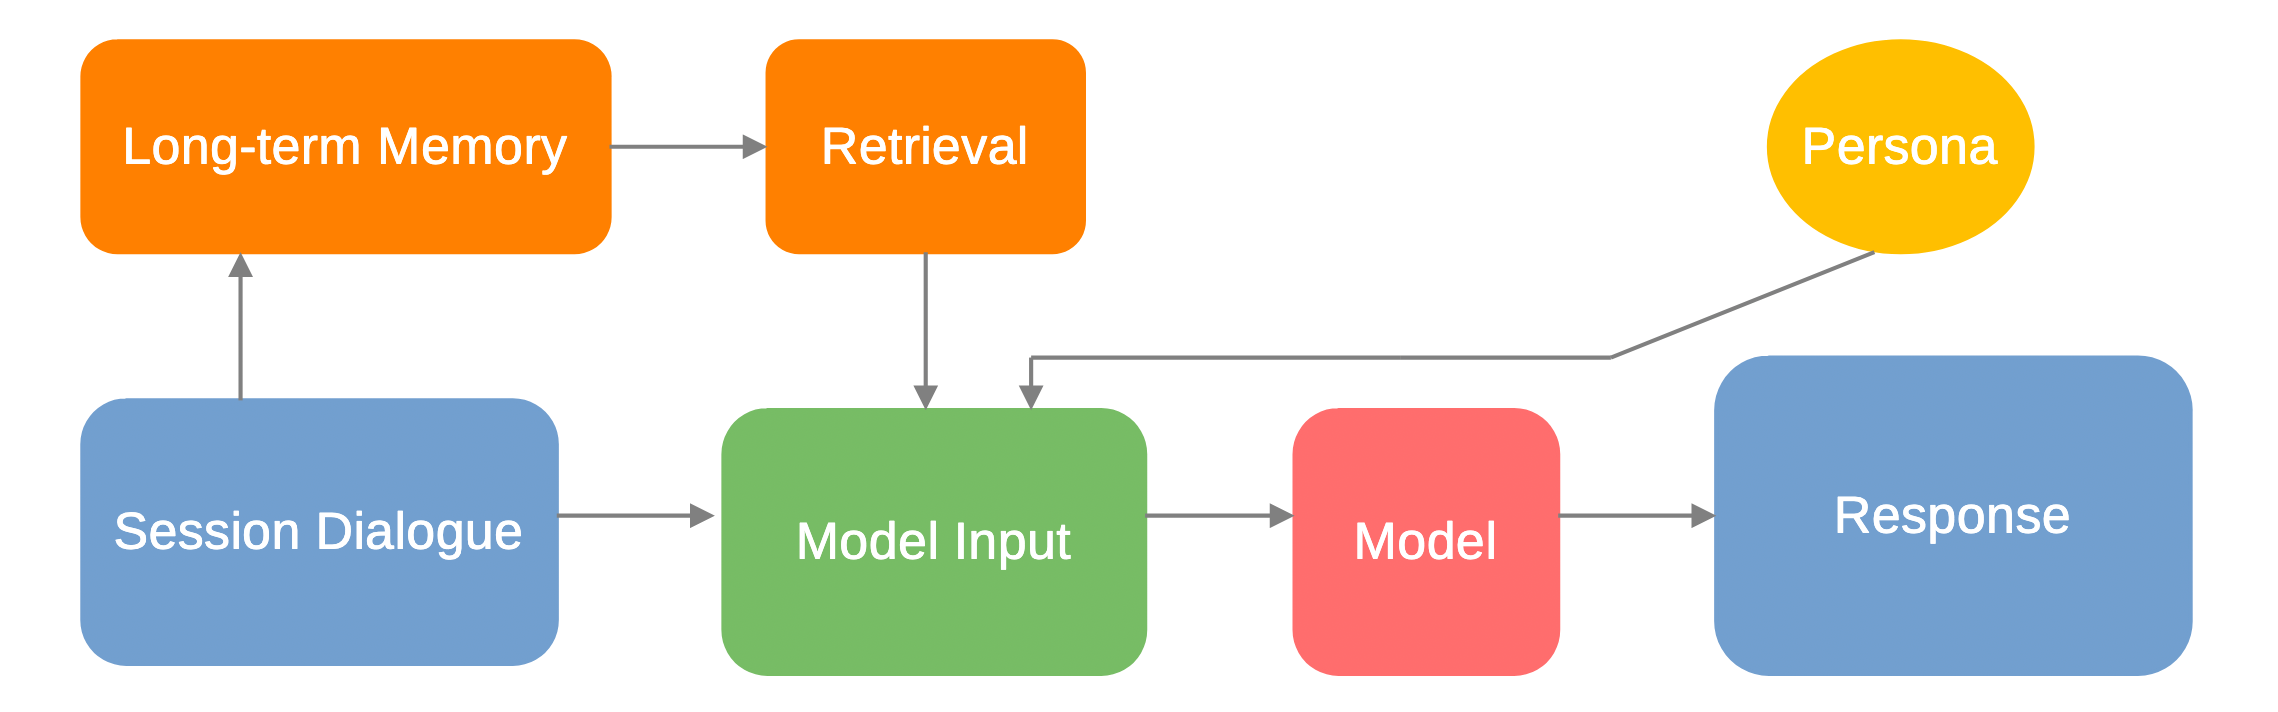
\includegraphics[width=1\textwidth]{images/pipeline}
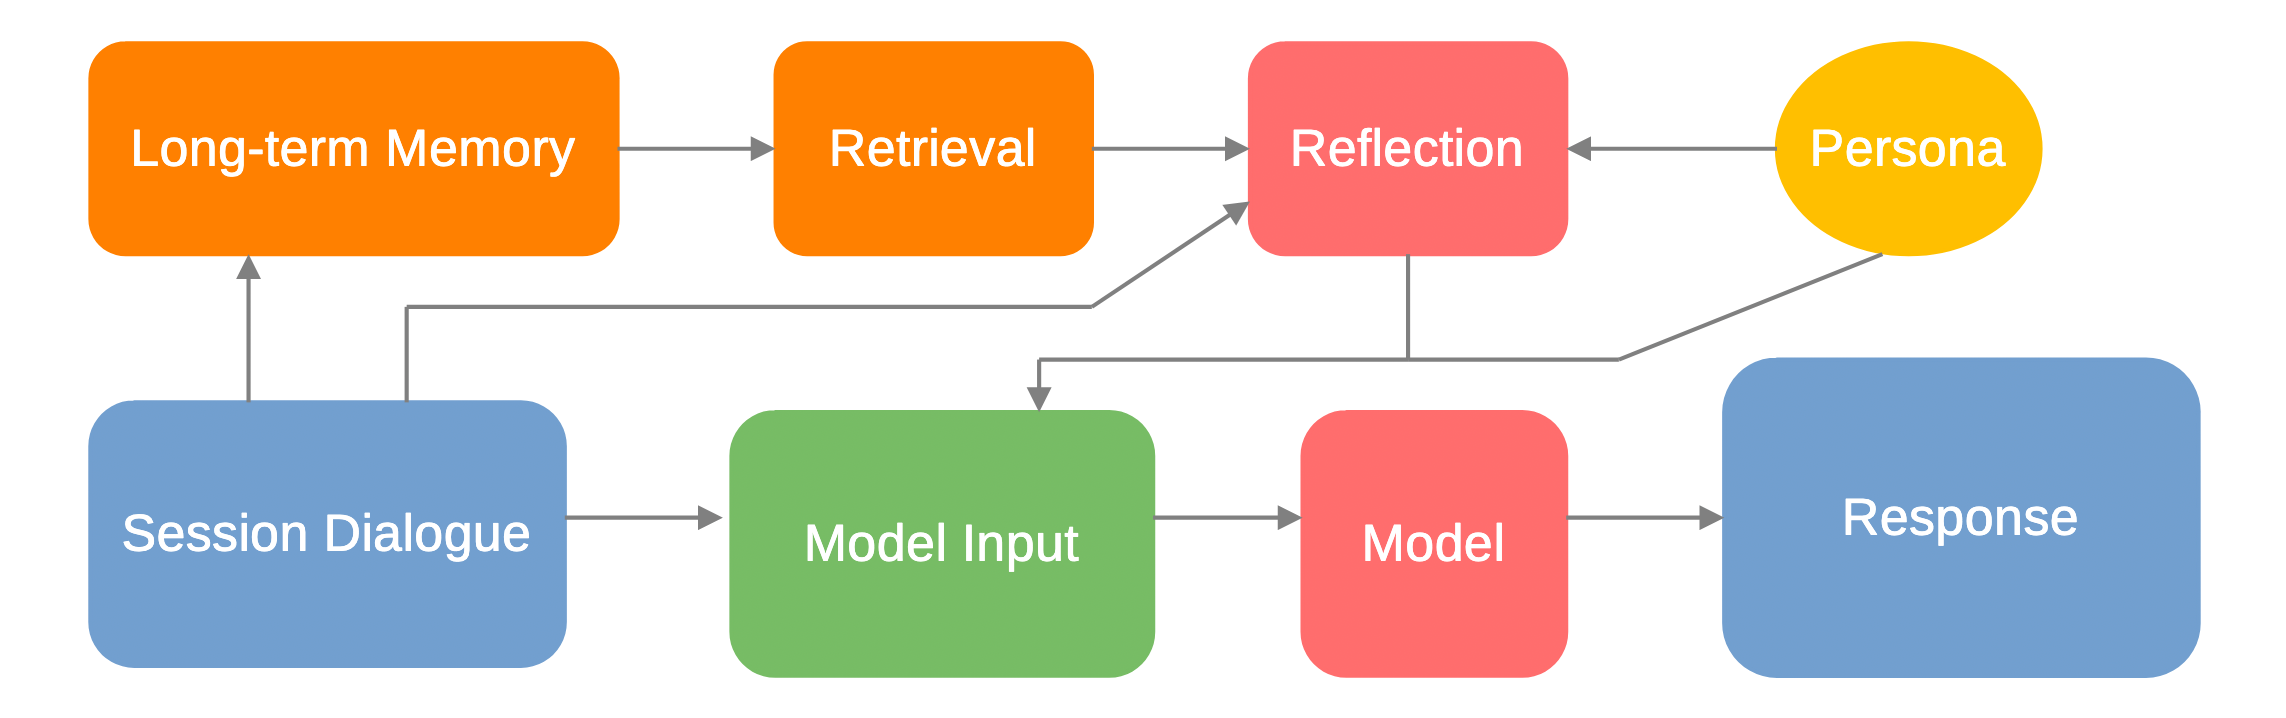
\includegraphics[width=1\textwidth]{images/pipeline_2}
\caption{The general conversational RAG pipeline, both with and without the reflection module}
\end{figure}